

\frame
{
\frametitle{
\includegraphics[width=.8cm]{images/books} References}

\begin{block}{Books}

\begin{itemize}
\item \alert{An Introduction to Bootstrap}, B. Efron and R. J. Tibshirani, Chapman \& Hall, 1998.
\item \alert{Bootstrap Methods and Their Application}, A. Davidson and D. Hinkley, Cambridge University Press, 1997.
\item \alert{Randomization, Bootstrapping, and Monte Carlo Methods in Biology}, Manly,   Chapman \& Hall, 1997.
\end{itemize}
\end{block}
\begin{block}{Special issues}
\begin{itemize}
\item \alert{Silver Anniversary of the Bootstrap}, Statistical Science, Vol. 18, nb. 2, May 2003.
\item \alert{Signal Processing Applications Of The Bootstrap} by S. Shamsunder; \alert {Computer-intensive methods in statistical analysis} by D.N. Politis;
\alert{The bootstrap and its application in signal processing}, A.M. Zoubir and B.  Boashash, in IEEE Signal Processing Magazine, January 1998.
\end{itemize}
\end{block}
}

%%%%%%%%%%%%%%%%%%%%%%%%%%%%%%%%%%%%%%%%%%%%%
\frame
{
\frametitle{The Empirical density function}

%Statistical inference concerns learning from experience: we observe 
Lets considerer  a  random sample (observations):
$$\mathbf{x}=(x_1,x_2,\cdots,x_n)$$ 

We wish to infer properties of the complete population $\mathcal{X}$ that yielded the sample. Lets define  the population density function $f(.)$ such that 
$$
f \leadsto \mathbf{x}=(x_1,x_2,\cdots,x_n) $$
%A complete knowledge is obtained from the  \alert{population density function}  $F(.)$ from which $\mathbf{x}$ has been generated  
%$F \leadsto \mathbf{x}=(x_1,x_2,\cdots,x_n) $

%\pause

\

\begin{definition}
The \alert{empirical density function} $\hat{f}(.)$ is defined as:
$$
{\textstyle\hat{f}(x)=\frac{1}{n}\sum_{i=1}^{n} \delta(x-x_i)}
%, \ \mathrm{where}
%\left\lbrace\begin{array}{l}
%\delta(x)=1,\  \mathrm{if}\ x=0\\
% \delta(x)=0,\  \mathrm{otherwise}\\
%\end{array}\right.
$$
where $\delta(\cdot)$ is the Dirac delta function.
%So the probability of $x=x_j$ is : 
%$$
%{\textstyle\int \hat{f}(x_j) \ dx = \int \ \frac{1}{n} \sum_{i=1}^{n} \delta(x_j-x_i)\  dx= 
%\left\lbrace
%\begin{array}{l}
%{\scriptstyle \frac{1}{n}, \ x_j\in\lbrace x_1,\cdots,x_n\rbrace}\\
%{\scriptstyle 0, \ \mathrm{otherwise}}\\
%\end{array}\right.
%}
%$$ 

\end{definition}
}

%%%%%%%%%%%%%%%%%%%%%%%%%%%%%%%%%%%%%%%%%%%%%%%%%%%%%%%%
\frame
{
\frametitle{Parameters}

\begin{definition}
A \alert{parameter}, $\theta$, is a function of the probability density function (p.d.f.) $f$, e.g.:
$$
\theta=t(f)
$$
\end{definition}
%\pause
\begin{exampleblock}{if $\theta$ is the mean}
%E.g.: if $\theta$ is the mean 
$$
\theta=\mathbb{E}_{f}(x) =\int_{-\infty}^{+\infty} x\ f(x) dx =\mu_f
$$
\end{exampleblock}
\begin{exampleblock}{if $\theta$ is the variance}
$$
\theta=\mathbb{E}_{f}\lbrack(x-\mu_f)^2\rbrack=\int_{-\infty}^{+\infty} (x-\mu_f)^2\ f(x) dx=\sigma_f^2
$$
\end{exampleblock}
}
\frame
{
\frametitle{Statistics or estimates}

\begin{definition}
A \alert{statistic} (also called estimates, estimators) $\hat{\theta}$ is a function of $\hat{f}$ or the sample $\mathbf{x}$, e.g.:
$$
\hat{\theta}=t(\hat{f})
$$
or also written $\hat{\theta}=s(\mathbf{x})$.
\end{definition}
\begin{exampleblock}{if $\hat{\theta}$ is the mean:}
%E.g.: if $\hat{\theta}$ is the mean:
$$
\begin{array}{llll}
\hat{\theta}&=t(\hat{f})&=\int_{-\infty}^{+\infty} x\ \hat{f}(x) dx & \\
&&&\\
&&=\int_{-\infty}^{+\infty} x\  \frac{1}{n}\sum_{i=1}^{n} \delta(x-x_i) \ dx&\\
&&&\\
&&= \frac{1}{n}\sum_{i=1}^{n} x_i &\\
&&&\\
&&=s(\mathbf{x})=\overline{x} &\\
\end{array}
$$
\end{exampleblock}
}
\frame
{
\frametitle{Statistics or estimates}
\begin{exampleblock}{if $\hat{\theta}$ is the variance:}
$$
\begin{array}{ll}
\hat{\theta}&=\int_{-\infty}^{+\infty} (x-\overline{x})^2\ \hat{f}(x) dx\\
&\\
&= \frac{1}{n}\sum_{i=1}^{n} (x_i-\overline{x})^{2}\\
&\\
&=\hat{\sigma}^{2}\\
\end{array}
$$ 

\end{exampleblock}
}


%%%%%%%%%%%%%%%%%%%%%%%%%%%%%%%%%%%%%%%%%%%%%%%%%%%%%%%%%%%%%
%\section{Plug-in Principle}
\frame
{
\frametitle{The Plug-in principle}
\begin{definition}
The \alert{Plug-in} estimate of a parameter $\theta=t(f)$ is defined to be:
$$ 
\hat{\theta}=t(\hat{f}).
$$ 
\small{The function $\theta=t(f)$ of the probability density function $f$ is estimated by the same  function $t(.)$ of the empirical density $\hat{f}$.}
\end{definition}

%\pause

\begin{exampleblock}{}
\begin{itemize}
\item $\overline{x}$ is the plug-in estimate of $\mu_f$.
\item $\hat{\sigma}$  is the plug-in estimate of $\sigma_f$
\end{itemize}
\end{exampleblock}
}
%%%%%%%%%%%%%%%%%%%%%%%%%%%%%%%%%%%%%%%%%%%%%%%%%%%%%%%%%%%%%
\frame
{
\frametitle{Computing the  mean knowing $f$}

\begin{exampleblock}{Example A}
\begin{columns}
\column[c]{.6\linewidth}
Lets assume we know the p.d.f. $f$: 
%\frac{\exp{\lbrack-\frac{(x-1)^2}{8}}\rbrack}{2\sqrt{2\pi}}
%\cdot \frac{\exp{\lbrack-\frac{(x-6)^2}{2}}\rbrack}{\sqrt{2\pi}}
$$
f(x)=0.2\ \mathcal{N}(\scriptstyle \mu=1,\sigma=2 \displaystyle) +0.8\  \mathcal{N}( \scriptstyle\mu=6,\sigma=1 \displaystyle)
$$
Then the mean  is computed:
$$
\begin{array}{ll}
\mu_{f}=\mathbb{E}_{f}(x)&=\int_{-\infty}^{+\infty} x\ f(x)\ dx \\
&\\
&=0.2\cdot 1 + 0.8 \cdot 6 \\
&\\
&=5\\
\end{array}
$$
\column[c]{.4\linewidth}
\begin{figure}[h!t]
\begin{center}
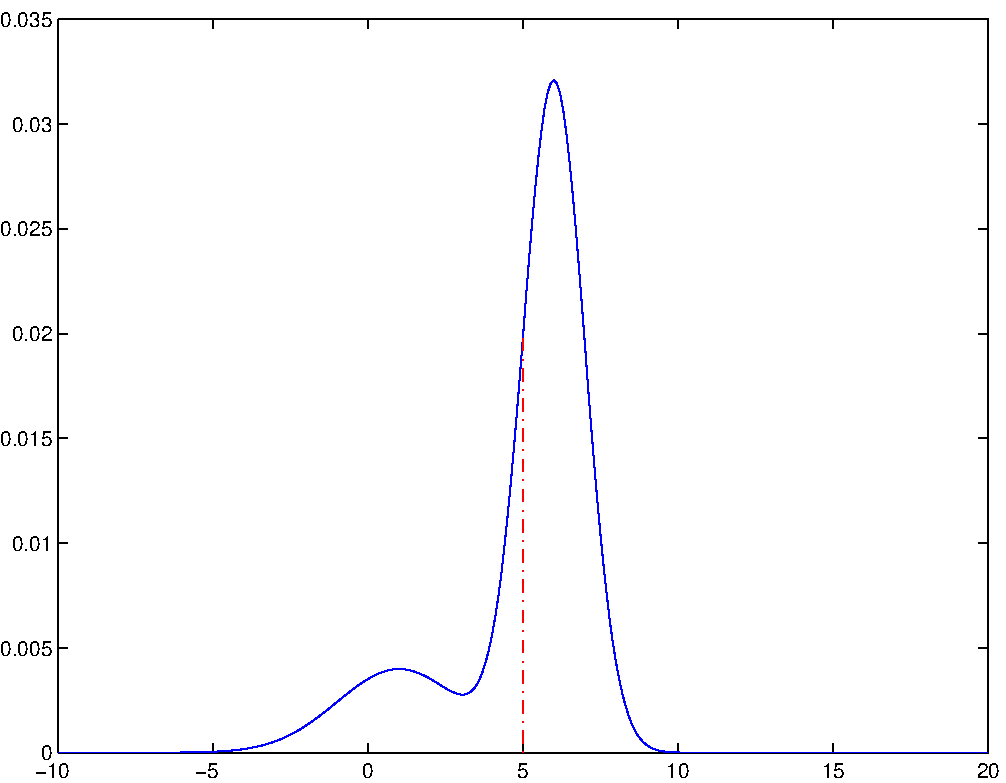
\includegraphics[width=.9\linewidth]{figure}
%\caption{\tiny{Distribution $f(x)$: $\mathbb{E}_{f}(x)=5$.}}
\end{center}
\end{figure}
\end{columns}
\end{exampleblock}
}
%%%%%%%%%%%%%%%%%%%%%%%%%%%%%%%%%%%%%%%%%%%%%%%%%%%%%%%%%%%%%
\frame
{
\frametitle{Estimating the mean knowing the observations $\mathbf{x}$}

\begin{exampleblock}{Example A}
\begin{columns}
\column[t]{.5\linewidth}
Observations $\mathbf{x}=(x_1,\cdots,x_{100})$ :
\tiny
$$
\left\lbrace
\begin{array}{ccccc}
   7.0411 &  4.8397 &  5.3156 &  6.7719 &  7.0616 \\
    5.2546 &   7.3937 &  4.3376 &   4.4010&    5.1724\\
    7.4199 &   5.3677 &  6.7028 &   6.2003 &   7.5707\\
    4.1230 &   3.8914 &   5.2323 &  5.5942 &    7.1479\\
  3.6790 &     0.3509 &   1.4197&   1.7585 &   2.4476\\
   -3.8635 &   2.5731 &   -0.7367 &  0.5627 &   1.6379\\
   -0.1864 &   2.7004 &   2.1487 &  2.3513 &   1.4833\\
   -1.0138 &  4.9794 &  0.1518 &  2.8683 &  1.6269 \\
    6.9523 & 5.3073 &  4.7191 &   5.4374 &   4.6108 \\
    6.5975 &  6.3495 & 7.2762 &  5.9453 &   4.6993\\
    6.1559&  5.8950 &  5.7591 &  5.2173 &   4.9980\\
    4.5010 &  4.7860 &  5.4382 &   4.8893&  7.2940\\
    5.5741 &  5.5139 &  5.8869 &  7.2756 &   5.8449 \\
    6.6439 &  4.5224 &  5.5028 &  4.5672 &  5.8718 \\
    6.0919 &  7.1912 &  6.4181 &  7.2248 &  8.4153 \\
    7.3199 &  5.1305 &  6.8719 &  5.2686 &   5.8055 \\
    5.3602 &  6.4120 &  6.0721 &  5.2740 &  7.2329\\
    7.0912 &  7.0766 &  5.9750 &  6.6091 &  7.2135 \\
    4.9585 &  5.9042 &  5.9273 &  6.5762 &   5.3702\\
    4.7654 &  6.4668 &  6.1983 &  4.3450 &   5.3261\\
\end{array}\right\rbrace
$$
\column[t]{.5\linewidth}
\normalsize
From the samples, the mean can be computed:
$$
\begin{array}{ll}
\overline{x}&=\frac{\sum_{i=1}^{100}x_i}{100}\\
&\\
&=  4.9970\\
\end{array}
$$
\end{columns}
\end{exampleblock}
}


%%%%%%%%%%%%%%%%%%%%%%%%%%%%%%%%%%%%%%%%%%%%%%%%%%%%
\frame
{
\frametitle{Accuracy of arbituary estimates $\hat{\theta}$}


We can compute an estimate $\hat{\theta}$ of a parameter $\theta$ from an observation sample $\mathbf{x}=(x_1,x_2,\cdots,x_n)$. But 

\

\alert{how accurate is $\hat{\theta}$ compared to the real value $\theta$ ?}

\

Our attention is focused on questions concerning the probability distribution of $\hat{\theta}$. For instance we would like to know about:
\begin{itemize}
\item its standard error
\item its confidence interval
\item its bias
\item etc. 
\end{itemize}

}

%%%%%%%%%%%%%%%%%%%%%%%%%%%%%%%%%%%%%%%%%%%%
%%%%%%%%%%%%%%%%%%%%%%%%%%%%%%%%%%%%%%%%%%%%%



%%%%%%%%%%%%%%%%%%%%%%%%%%%%%%%%%%%%%%%%%%%%
\frame
{
\frametitle{Standard error of $\hat{\theta}$}
\begin{definition}
The \alert{standard error} is the standard deviation  of a statistic $\hat{\theta}$. As such, it measures the precision of an estimate of the statistic  of a population distribution.
$$
se(\hat{\theta})=\sqrt{var_{f}{[\hat{\theta}]}}
$$
\end{definition}

%\pause

\begin{exampleblock}{Standard error of  $\overline{x}$}
We have:
$$
\mathbb{E}_{f}\left\lbrack (\overline{x}-\mu_f)^2\right\rbrack=% \mathbb{E}_{f}\left\lbrack \left(\frac{\sum_{i=1}^n (x_i-\mu_{f})}{n}\right)^2\right\rbrack =
\frac{\sum_{i=1}^n \mathbb{E}_{f}\left\lbrack (x_i-\mu_{f})^2\right\rbrack}{n^2}=\frac{\sigma_{f}^{2}}{n}
$$
Then
$$
se_{f}(\overline{x})=\lbrack\mathrm{var}_{f}(\overline{x})\rbrack^{1/2}=\frac{\sigma_{f}}{\sqrt{n}}
$$

\end{exampleblock}
}


%%%%%%%%%%%%%%%%%%%%%%%%%%%%%%%%%%%%%%%%%%%%
\frame
{
\frametitle{Plug in estimate of the standard error}

Suppose now that $f$ is unknown and that only the random sample $\mathbf{x}=(x_1,\cdots,x_n)$ is known.
As $\mu_f$ and $\sigma_f$ are unknown, we can use the previous formula to compute a plug-in estimate of the  standard error.
\begin{definition}
The \alert{estimated standard error} of the estimator $\hat{\theta}$ is defined as:
$$
\hat{\mathrm{se}}(\hat{\theta})=\mathrm{se}_{\hat{f}}(\hat{\theta})=\lbrack\mathrm{var}_{\hat{f}}(\hat{\theta})\rbrack^{1/2}
$$
\end{definition}

%\pause

\begin{exampleblock}{Estimated standard error of $\overline{x}$ }
$$
\hat{\mathrm{se}} (\overline{x})=\frac{\hat{\sigma}}{\sqrt{n}}
$$
\end{exampleblock}
}

%%%%%%%%%%%%%%%
\frame
{
\frametitle{Example on the mouse data}

\begin{table}[!h]
\begin{tabular}{|c|c|}
\hline
&\\
 Data (Treatment group) & 94; 197; 16; 38; 99; 141; 23 \\
&\\
\hline
& \\
Data (Control group) & 52; 104; 146; 10; 51; 30; 40; 27; 46 \\
& \\
\hline
\end{tabular}
\caption{The mouse data [Efron]. 16 mice  assigned to a treatment group (7) or a control group (9). Survival in days following a test surgery.  }
\end{table}

\centering{\alert{\textbf{Did the treatment prolong survival ?}}}


}

\frame
{
\frametitle{Example on the mouse data}



\begin{exampleblock}{Mean and Standard error for both groups}
%Using the formulas, we have $\overline{x}_{Treat}=86.86$ and $\hat{\mathrm{se}}_{Treat}(\overline{x})=25.24$
%and $\overline{x}_{Cont}=56.22$ and $\hat{\mathrm{se}}_{Cont}(\overline{x})=14.14$. 
\begin{table}[!h]
\begin{tabular}{c|c|c}
& $\overline{x}$ & $\hat{\mathrm{se}} $ \\
\hline
Treatment & 86.86 & 25.24 \\
\hline
Control & 56.22 & 14.14 \\
\end{tabular}
\end{table}
\end{exampleblock}


\begin{block}{Conclusion at first glance} 
It seems that mice having the treatment survive $d=86.86-56.22=30.63$ days more than the mice from the control group.
\end{block}



}


\frame
{
\frametitle{Example on the mouse data}


\begin{exampleblock}{Stantard error of the difference $d=\overline{x}_{Treat}-\overline{x}_{Cont}$}
$\overline{x}_{Treat}$ and $\overline{x}_{Cont}$ are independent, so the standard error of their difference is $\hat{\mathrm{se}}(d)=\sqrt{\hat{\mathrm{se}}_{Treat}^2 +\hat{\mathrm{se}}_{Cont}^2 }=28.93$. 
We see that:
$$
\frac{d}{\hat{\mathrm{se}}(d)}
=\frac{30.63}{28.93}=1.05
 $$
This shows that this is an insignificant result as it could easily have arised by chance (i.e. if the test was reproduced, it is \textit{likely possible} to measure datasets giving $d=0$!).  

Therefore, we can not conclude with certainty that the treatment improves the survival of the mice.
\end{exampleblock}
}



%%%%%%%%%%%%%%%%%%%%%%%%%%%%%%%%%%%%%%%%%%%%
\frame
{
\frametitle{Confidence interval for $\hat{\theta}$}


\begin{definition}

Assuming that the estimator $\hat{\theta}$ is normally distributed with unknown expectation $\theta$ and variance $\mathrm{se}^2$, then :

$$
\mathrm{Prob}\lbrace \hat{\theta}-z^{(1-\alpha)} \mathrm{se}\leq  \theta \leq \hat{\theta}- z^{(\alpha)} \mathrm{se}\rbrace=1-2\alpha
$$
Therefore   $1-2\alpha$ \% \alert{confidence interval} for $\theta$ is
$
\lbrack \hat{\theta}-z^{(1-\alpha)}\mathrm{se} ; \hat{\theta}- z^{(\alpha)} \mathrm{se}\rbrack
$

\alert{Confidence limits} are the lower and upper boundaries  values of a confidence interval. The \alert{confidence level} is the probability value $100 \times (1-2\alpha)$ \% associated with a confidence interval.

\end{definition}


}
%%%%%%%%%%%%%%%%%%%%%%%%%%%%%%%%%%%%%%%%%%%%%
\frame
{
\frametitle{Confidence interval}

The width of the confidence interval gives us some idea about how uncertain we are about the unknown parameter. A very wide interval may indicate that more data should be collected before anything very definite can be said about the parameter.

\begin{columns}
\column[t]{0.5\linewidth}
\begin{table}[!h]
\begin{tabular}{|c|c|c|}
\hline
\tiny{percentile} &\tiny{confidence level}& \\
$\alpha\times 100$ \% & $(1-2\alpha)\times 100$  \% & $z^{(1-\alpha)}$\\
\hline
10 &80 & $1.28155 $ \\	
5 & 90 &	$1.64485$ \\
2.5 & 95 	& $1.95996 $ \\
0.5 & 99 	& $2.57583 $ \\
0.25 &99.5 	& $2.80703 $ \\
0.05 &99.9 	& $3.29053 $ \\
\hline
\end{tabular}
\caption{\tiny{For a normal p.d.f $z^{(\alpha)}=-z^{(1-\alpha)}$}}
\end{table}
\column[t]{0.5\linewidth}
\begin{figure}[!h]
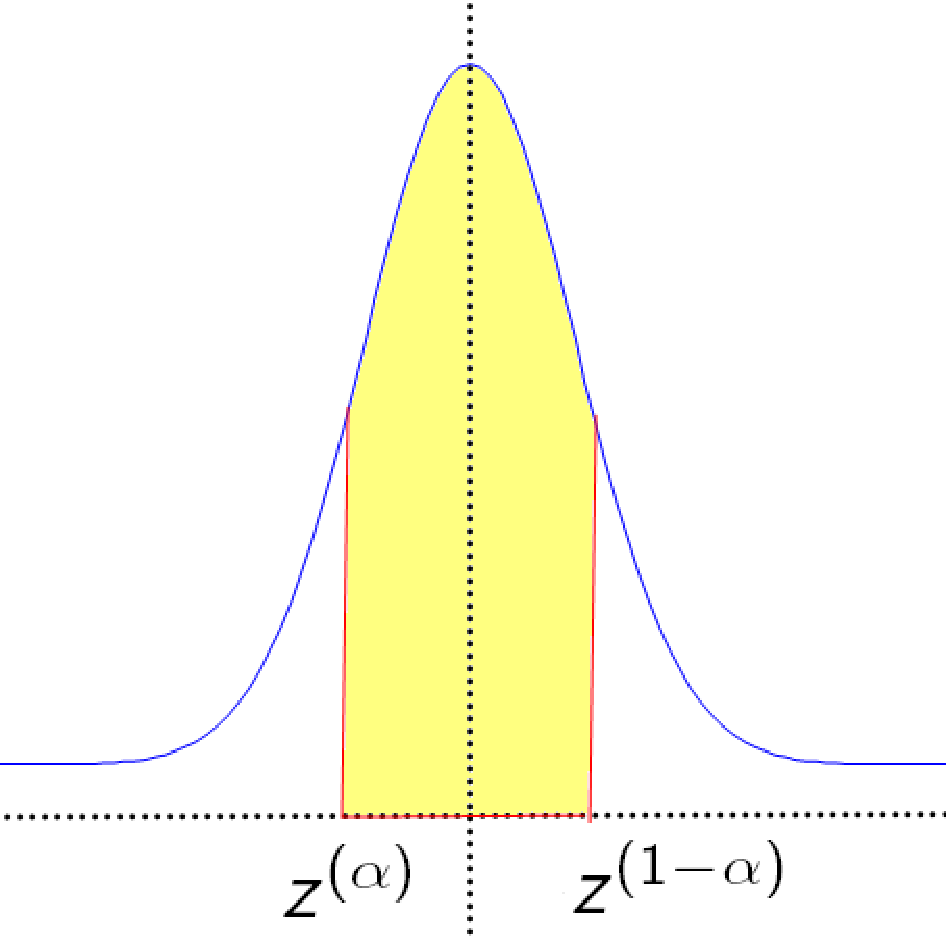
\includegraphics[width=.6\linewidth]{gaussien.pdf}
\caption{ \tiny{Density function $\mathcal{N}(0,1)$.}}
\end{figure}
\end{columns}
}
%%%%%%%%%%%%%%%%%%%%%%%%%%%%%%%%%%%%%%%%%%
\frame
{
\frametitle{Example Confidence interval}

\begin{exampleblock}{Confidence interval of the mean}
Using the central limit theorem, the estimate  $\overline{x}$ is following a normal density function $\mathcal{N}\left(\mu_f,\frac{\sigma_f^2}{n}\right)$.
The 90\% confidence interval is :
$$
\overline{x}\pm 1.645 \frac{\sigma_f}{\sqrt{n}}\  \mathrm{estimated\ by} \pm 1.645 \frac{\hat{\sigma}}{\sqrt{n}}
$$
\end{exampleblock}

\begin{exampleblock}{confidence interval of the difference for the mouse data}
The difference $d$ in days of survival between the treatment group and the control group has a estimated 90\% confidence interval defined as:
$$
 d=30.63\pm  1.645\times 28.93=30.63 \pm 47.5898 
$$
\end{exampleblock}
}
%%%%%%%%%%%%%%%%%%%%%%%%%%%%%%%%%%%%%%%%%%
\frame
{
\frametitle{Bias of $\hat{\theta}$}
\begin{definition}
The \alert{Bias} is the difference between the expectation of an estimator $\hat{\theta}$ and the quantity $\theta$ being estimated:
$$
\mathrm{Bias}_{f}(\hat{\theta},\theta)=\mathbb{E}_f(\hat{\theta})-\theta
$$
\end{definition}


 \begin{exampleblock}{Bias of the mean $\overline{x}$}
we have:
$$
\mathbb{E}_{f}(\overline{x})=\mathbb{E}_{f}\left(\frac{\sum_{i=1}^{n} x_i}{n}\right)=\frac{\sum_{i=1}^{n}\mathbb{E}_{f}( x_i)}{n}=\mu_f
$$
then:
$$
\mathrm{Bias}_{f}(\overline{x},\mu_f)=\mathbb{E}_f(\overline{x})-\mu_f =0
$$
\end{exampleblock}
}

%% lots of mistakes -
\frame
{
\frametitle{Bias of $\hat{\theta}$}

\begin{itemize}
\item A large bias is usually an undesirable aspect of an estimator's performance. \alert{Unbiased estimates} (such $\mathbb{E}_f(\hat{\theta})=\theta$) are interesting in practice as they promote a nice feeling of scientific objectivity in the estimation process. 
%\item Plug- in estimates $\hat{\theta}=t(\hat{f})$ are not necessarily unbiased but they tend to have small biases compared to the magnitude of their standard error.
\end{itemize}

\begin{exampleblock}{Bias of $\hat{\sigma}^2$}
$$
\begin{array}{ll}
\hat{\sigma}^2&=\frac{1}{n} \sum_{i=1}^{n} (x_i-\overline{x})^{2}=\frac{1}{n} \sum_{i=1}^{n} ((x_i-\mu_f)+ (\mu_f-\overline{x}))^{2}\\
&\\
&=\left(\frac{1}{n}  \sum_{i=1}^{n} (x_i-\mu_f)^2 \right)-  (\overline{x}-\mu_f)^2\\
\end{array}
$$
The first term has an expected value of $\sigma_f^2$ and the second term has expected value $\sigma_f^2/n$. So the bias of  $\hat{\sigma}^2$ is:
$$
\mathrm{Bias}_{f}(\hat{\sigma}^2,\sigma_f^2)=\sigma_f^2-\frac{\sigma_f^2}{n}-\sigma_f^2=-\frac{\sigma_f^2}{n}
$$ 
\end{exampleblock}
}

%% lots of mistakes -
\frame
{
\frametitle{Bias of $\hat{\theta}$}

Instead of using $\hat{\sigma}^2$ as an estimate of the variance, you should try to choose an unbiased estimate. 

\begin{exampleblock}{Bias of $\overline{\sigma}^2$}
Let define:
$$ 
\overline{\sigma}^2=\frac{1}{n-1} \sum_{i=1}^{n} (x_i-\overline{x})^{2}
$$
then by computing its bias:
$$
\begin{array}{ll}
\mathrm{Bias}_f(\overline{\sigma}^2,\sigma_f^2)&=\mathbb{E}_{f}(\overline{\sigma}^2)-\sigma_f^2\\
&=0\\
\end{array}
$$
$\overline{\sigma}$ is an unbiased estimator of the standard deviation.
\end{exampleblock}


}

%%%%%%%%%%%%%%%%%%%%%%%%%%%%%%%%%%%%%%%%%%
\frame{
\frametitle{Summary }


\begin{itemize}
\item Population density function $f(\cdot)$ and empirical density function $\hat{f}(\cdot)$, 

\

\item Plug-in principle: relation between $\theta$ and its estimate $\hat{\theta}$ 

\

\item Standard error and confidence interval as a measure of accuracy of the estimate $\hat{\theta}$ 

\

\item Accuracy of estimate is important to draw conclusions (e.g. mouse example). 

\

\item se has an explicit expression for the mean $\overline{x}$
\end{itemize}

}

\frame{
\frametitle{Open problems}

\begin{itemize}
\item $f$ is generally unknown! 

\

\item Using the Plug-in principle, with more samples $\lbrace \mathbf{x} \rbrace$ drawn from $f$, we could estimate $\hat{se}$ or the bias.

\

\item But the only information available is one sample $\mathbf{x}=(x_1, \cdot,x_n)$ drawn from $f$! 

\

\item Most of all, explicit expression of $\mathrm{se}$ of the estimate is not easy to get in most cases!

\end{itemize}

}
